\newpage
\subsection{Caso d'uso UC7 - Visualizzazione API}
\label{UC7}
\begin{figure}[ht]
	\centering
	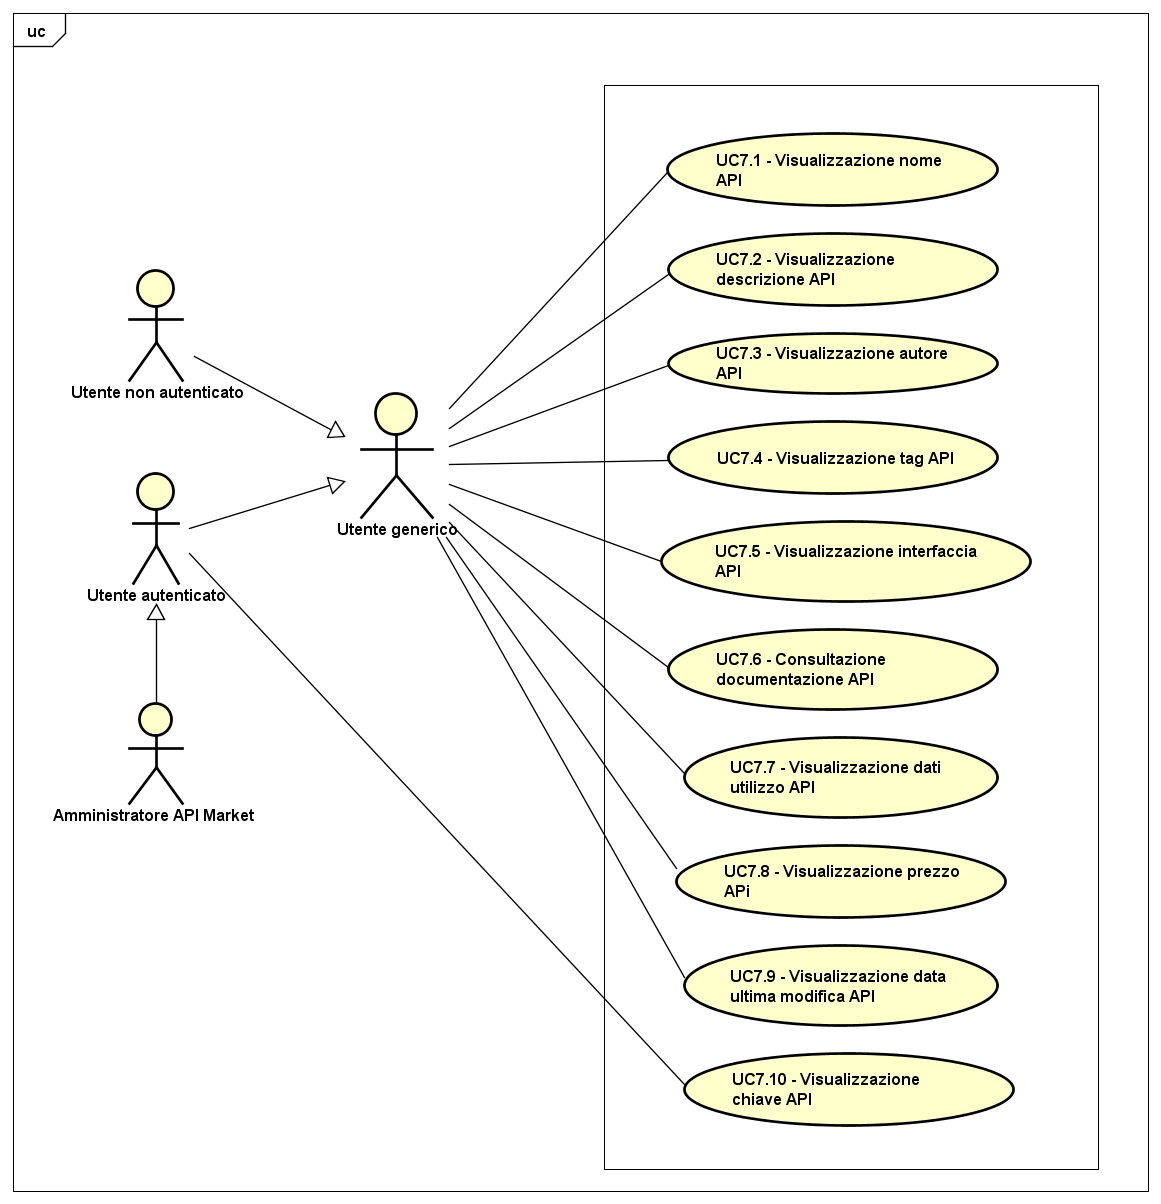
\includegraphics[scale=0.45]{UML/UC7.png}
	\caption{UC7: Visualizzazione API}
\end{figure}

\begin{longtable}{ l | p{11cm}}
	\hline
	\rowcolor{Gray}
	\multicolumn{2}{c}{UC7 - Visualizzazione API}\\
	\hline
	
	 \textbf{Attori} & Utente non autenticato, Utente autenticato  \\
	\textbf{Descrizione} & L'attore può visualizzare i dati relativi a un API che ha selezionato tramite la homepage o i risultati di una ricerca  \\
	\textbf{Pre-Condizioni} & L'attore ha selezionato un prodotto per la consultazione \\
	\textbf{Post-Condizioni} & L'attore visualizza la pagina relativa all'API selezionata\\
	\textbf{Scenario Principale} & 
	\begin{enumerate*}[label=(\arabic*.),itemjoin={\newline}]
		\item L'attore visualizza il nome dell'API (UC7.1)
		\item L'attore visualizza la descrizione dell'API (UC7.2)
		\item L'attore visualizza l'autore dell'API (UC7.3)
		\item L'attore visualizza i tag registrati relativi all'API (UC7.4)
		\item L'attore può visualizzare l'interfaccia dell'API (UC7.5)
		\item L'attore può consultare la documentazione fornita dall'utente (UC7.6)
		\item L'attore può visualizzare i dati di utilizzo dell'API  (UC7.7)
		\item L'attore può acquistare l'API visualizzata (UC9)
	\end{enumerate*}\\
	\textbf{Scenari Alternativi} & 
	\begin{enumerate*}[label=(\arabic*.),itemjoin={\newline}]
		\item L'attore possiede una licenza attiva per il prodotto, e può visualizzarne la chiave personale di utilizzo (UC7.8)
	\end{enumerate*}\\
\end{longtable}


\subsubsection{Caso d'uso UC7.1: Visualizzazione nome API}
\label{UC7_1}

\begin{minipage}{\linewidth}
	\begin{tabular}{ l | p{11cm}}
		\hline
		\rowcolor{Gray}
		\multicolumn{2}{c}{UC7.1 - Visualizza nome API} \\
		\hline
		\textbf{Attori} & Utente non autenticato, Utente autenticato \\
		\textbf{Descrizione} & L'attore visualizza il nome dell'API nella schermata relativa\\
		\textbf{Pre-Condizioni} & L'attore ha selezionato un API per poterla visualizzare\\
		\textbf{Post-Condizioni} & L'attore visualizza il nome dell'API selezionata \\
		\textbf{Scenario Principale} & 
		\begin{enumerate*}[label=(\arabic*.),itemjoin={\newline}]
			\item L'attore può visualizzare il nome dell'API selezionata
		\end{enumerate*}\\
	\end{tabular}
\end{minipage}

\subsubsection{Caso d'uso UC7.2: Visualizzazione descrizione API}
\label{UC7_2}

\begin{minipage}{\linewidth}
	\begin{tabular}{ l | p{11cm}}
		\hline
		\rowcolor{Gray}
		\multicolumn{2}{c}{UC7.2 - Visualizzazione descrizione API} \\
		\hline
		\textbf{Attori} & Utente non autenticato, Utente autenticato \\
		\textbf{Descrizione} & L'attore visualizza la descrizione dell'API nella schermata relativa\\
		\textbf{Pre-Condizioni} & L'attore ha selezionato un API per poterla visualizzare\\
		\textbf{Post-Condizioni} & L'attore visualizza la descrizione dell'API selezionata \\
		\textbf{Scenario Principale} & 
		\begin{enumerate*}[label=(\arabic*.),itemjoin={\newline}]
			\item L'attore può visualizzare la descrizione dell'API selezionata
		\end{enumerate*}\\
	\end{tabular}
\end{minipage}

\subsubsection{Caso d'uso UC7.3: Visualizzazione autore API}
\label{UC7_3}

\begin{minipage}{\linewidth}
	\begin{tabular}{ l | p{11cm}}
		\hline
		\rowcolor{Gray}
		\multicolumn{2}{c}{UC7.3 - Visualizzazione autore API} \\
		\hline
		\textbf{Attori} & Utente non autenticato, Utente autenticato \\
		\textbf{Descrizione} & L'attore visualizza il nome dell'autore dell'API nella schermata relativa\\
		\textbf{Pre-Condizioni} & L'attore ha selezionato un API per poterla visualizzare\\
		\textbf{Post-Condizioni} & L'attore visualizza il nome dell'autore per l'API selezionata \\
		\textbf{Scenario Principale} & 
		\begin{enumerate*}[label=(\arabic*.),itemjoin={\newline}]
			\item L'attore può visualizzare il nome dell'autore per l'API selezionata
		\end{enumerate*}\\
	\end{tabular}
\end{minipage}

\subsubsection{Caso d'uso UC7.4: Visualizzazione tag API}
\label{UC7_4}

\begin{minipage}{\linewidth}
	\begin{tabular}{ l | p{11cm}}
		\hline
		\rowcolor{Gray}
		\multicolumn{2}{c}{UC7.4 - Visualizzazione tag API} \\
		\hline
		\textbf{Attori} & Utente non autenticato, Utente autenticato \\
		\textbf{Descrizione} & L'attore visualizza i tag dell'API nella schermata relativa\\
		\textbf{Pre-Condizioni} & L'attore ha selezionato un API per poterla visualizzare\\
		\textbf{Post-Condizioni} & L'attore visualizza i tag per l'API selezionata \\
		\textbf{Scenario Principale} & 
		\begin{enumerate*}[label=(\arabic*.),itemjoin={\newline}]
			\item L'attore può visualizzare i tag assegnati all'API selezionata
		\end{enumerate*}\\
	\end{tabular}
\end{minipage}

\subsubsection{Caso d'uso UC7.5: Visualizzazione interfaccia API}
\label{UC7_5}

\begin{minipage}{\linewidth}
	\begin{tabular}{ l | p{11cm}}
		\hline
		\rowcolor{Gray}
		\multicolumn{2}{c}{UC7.5 - Visualizzazione interfaccia API} \\
		\hline
		\textbf{Attori} & Utente non autenticato, Utente autenticato \\
		\textbf{Descrizione} & L'attore visualizza l'interfaccia dell'API nella schermata relativa\\
		\textbf{Pre-Condizioni} & L'attore ha selezionato un API per poterla visualizzare\\
		\textbf{Post-Condizioni} & L'attore visualizza l'interfaccia dell'API selezionata \\
		\textbf{Scenario Principale} & 
		\begin{enumerate*}[label=(\arabic*.),itemjoin={\newline}]
			\item L'attore può visualizzare l'interfaccia dell'API selezionata
		\end{enumerate*}\\
	\end{tabular}
\end{minipage}

\subsubsection{Caso d'uso UC7.6: Visualizzazione documentazione API}
\label{UC7_6}

\begin{minipage}{\linewidth}
	\begin{tabular}{ l | p{11cm}}
		\hline
		\rowcolor{Gray}
		\multicolumn{2}{c}{UC7.6 - Visualizzazione documentazione API} \\
		\hline
		\textbf{Attori} & Utente non autenticato, Utente autenticato \\
		\textbf{Descrizione} & L'attore può visualizzare la documentazione dell'API\\
		\textbf{Pre-Condizioni} & L'attore ha selezionato un API per poterla visualizzare\\
		\textbf{Post-Condizioni} & L'attore visualizza la documentazione dell'API selezionata \\
		\textbf{Scenario Principale} & 
		\begin{enumerate*}[label=(\arabic*.),itemjoin={\newline}]
			\item L'attore può visualizzare la documentazione dell'API selezionata tramite un link esterno fornita dall'autore (UC7.6.1)
			\item L'attore può visualizzare la documentazione dell'API selezionata scaricando il file PDF fornito dall'autore (UC7.6.2)
		\end{enumerate*}\\
	\end{tabular}
\end{minipage}

\subsubsection{Caso d'uso UC7.6.1: Visualizzazione esterna documentazione}
\label{UC7_6_1}

\begin{minipage}{\linewidth}
	\begin{tabular}{ l | p{11cm}}
		\hline
		\rowcolor{Gray}
		\multicolumn{2}{c}{UC7.6.1 - Visualizzazione esterna documentazione} \\
		\hline
		\textbf{Attori} & Utente non autenticato, Utente autenticato, Pagina web esterna \\
		\textbf{Descrizione} & L'attore può visualizzare la documentazione dell'API tramite un link esterno fornito dall'autore\\
		\textbf{Pre-Condizioni} & L'attore visualizza un link relativo alla documentazione esterna\\
		\textbf{Post-Condizioni} & L'attore apre il link, e viene reindirizzato ad una pagina esterna fornita dall'autore dell'API \\
		\textbf{Scenario Principale} & 
		\begin{enumerate*}[label=(\arabic*.),itemjoin={\newline}]
			\item L'attore visita la pagina esterna per consultare la documentazione fornita dall'autore
		\end{enumerate*}\\
	\end{tabular}
\end{minipage}

\subsubsection{Caso d'uso UC7.6.2: Scarica documentazione PDF}
\label{UC7_6_2}

\begin{minipage}{\linewidth}
	\begin{tabular}{ l | p{11cm}}
		\hline
		\rowcolor{Gray}
		\multicolumn{2}{c}{UC7.6.2 - Scarica documentazione PDF} \\
		\hline
		\textbf{Attori} & Utente non autenticato, Utente autenticato \\
		\textbf{Descrizione} & L'attore può scaricare la documentazione dell'API in formato PDF\\
		\textbf{Pre-Condizioni} & L'attore visualizza un link relativo alla documentazione in PDF\\
		\textbf{Post-Condizioni} & L'attore seleziona il link di download e scarica la documentazione in formato PDF \\
		\textbf{Scenario Principale} & 
		\begin{enumerate*}[label=(\arabic*.),itemjoin={\newline}]
			\item L'attore può scaricare la documentazione fornita dall'autore dell'API in formato PDF
		\end{enumerate*}\\
	\end{tabular}
\end{minipage}

\subsubsection{Caso d'uso UC7.7: Visualizzazione dati utilizzo API}
\label{UC7_7}

\begin{minipage}{\linewidth}
	\begin{tabular}{ l | p{11cm}}
		\hline
		\rowcolor{Gray}
		\multicolumn{2}{c}{UC7.7 - Visualizzazione dati utilizzo API} \\
		\hline
		\textbf{Attori} & Utente non autenticato, Utente autenticato \\
		\textbf{Descrizione} & L'attore visualizza i dati di utilizzo dell'API nella schermata relativa\\
		\textbf{Pre-Condizioni} & L'attore ha selezionato un API per poterla visualizzare\\
		\textbf{Post-Condizioni} & L'attore visualizza i dati di utilizzo per l'API selezionata \\
		\textbf{Scenario Principale} & 
		\begin{enumerate*}[label=(\arabic*.),itemjoin={\newline}]
			\item L'attore può visualizzare il numero di licenze attive (UC7.7.1)
			\item L'attore può visualizzare il numero di chiamate giornaliere effettuate (UC7.7.2)
			\item L'attore può visualizzare il tempo medio di utilizzo (UC7.7.3)
			\item L'attore può visualizzare il quantitativo di dati scambiati (UC7.7.4)
		\end{enumerate*}\\
	\end{tabular}
\end{minipage}

\subsubsection{Caso d'uso UC7.7.1: Visualizzazione licenze attive}
\label{UC7_7.1}

\begin{minipage}{\linewidth}
	\begin{tabular}{ l | p{11cm}}
		\hline
		\rowcolor{Gray}
		\multicolumn{2}{c}{UC7.7.1 - Visualizzazione licenze attive} \\
		\hline
		\textbf{Attori} & Utente non autenticato, Utente autenticato \\
		\textbf{Descrizione} & L'attore visualizza il numero di licenze attive \\
		\textbf{Pre-Condizioni} & L'attore si trova nella schermata relativa ad una singola API\\
		\textbf{Post-Condizioni} & L'attore visualizza il numero di licenze attive per l'API selezionata \\
		\textbf{Scenario Principale} & 
		\begin{enumerate*}[label=(\arabic*.),itemjoin={\newline}]
			\item L'attore può visualizzare il numero di licenze attive per l'API selezionata
		\end{enumerate*}\\
	\end{tabular}
\end{minipage}

\subsubsection{Caso d'uso UC7.7.2: Visualizzazione chiamate giornaliere}
\label{UC7_7.2}

\begin{minipage}{\linewidth}
	\begin{tabular}{ l | p{11cm}}
		\hline
		\rowcolor{Gray}
		\multicolumn{2}{c}{UC7.7.2 - Visualizzazione chiamate giornaliere} \\
		\hline
		\textbf{Attori} & Utente non autenticato, Utente autenticato \\
		\textbf{Descrizione} & L'attore visualizza il numero di chiamate giornaliere \\
		\textbf{Pre-Condizioni} & L'attore si trova nella schermata relativa ad una singola API\\
		\textbf{Post-Condizioni} & L'attore visualizza il numero di chiamate giornaliere per l'API selezionata \\
		\textbf{Scenario Principale} & 
		\begin{enumerate*}[label=(\arabic*.),itemjoin={\newline}]
			\item L'attore può visualizzare il numero di chiamate giornaliere per l'API selezionata
		\end{enumerate*}\\
	\end{tabular}
\end{minipage}

\subsubsection{Caso d'uso UC7.7.3: Visualizzazione tempo medio di utilizzo}
\label{UC7_7.3}

\begin{minipage}{\linewidth}
	\begin{tabular}{ l | p{11cm}}
		\hline
		\rowcolor{Gray}
		\multicolumn{2}{c}{UC7.7.3 - Visualizzazione tempo medio di utilizzo} \\
		\hline
		\textbf{Attori} & Utente non autenticato, Utente autenticato \\
		\textbf{Descrizione} & L'attore visualizza il tempo medio di utilizzo \\
		\textbf{Pre-Condizioni} & L'attore si trova nella schermata relativa ad una singola API\\
		\textbf{Post-Condizioni} & L'attore visualizza il tempo medio di utilizzo per l'API selezionata \\
		\textbf{Scenario Principale} & 
		\begin{enumerate*}[label=(\arabic*.),itemjoin={\newline}]
			\item L'attore può visualizzare il tempo medio di utilizzo per l'API selezionata
		\end{enumerate*}\\
	\end{tabular}
\end{minipage}

\subsubsection{Caso d'uso UC7.7.4: Visualizzazione dati scambiati}
\label{UC7_7.4}

\begin{minipage}{\linewidth}
	\begin{tabular}{ l | p{11cm}}
		\hline
		\rowcolor{Gray}
		\multicolumn{2}{c}{UC7.7.4 - Visualizzazione dati scambiati} \\
		\hline
		\textbf{Attori} & Utente non autenticato, Utente autenticato \\
		\textbf{Descrizione} & L'attore visualizza il quantitativo di dati scambiati tra l'utilizzatore e il microservizio \\
		\textbf{Pre-Condizioni} & L'attore si trova nella schermata relativa ad una singola API\\
		\textbf{Post-Condizioni} & L'attore visualizza il quantitativo di dati scambiati per l'API selezionata \\
		\textbf{Scenario Principale} & 
		\begin{enumerate*}[label=(\arabic*.),itemjoin={\newline}]
			\item L'attore può visualizzare il quantitativo di dati scambiati per l'API selezionata
		\end{enumerate*}\\
	\end{tabular}
\end{minipage}

\subsubsection{Caso d'uso UC7.8: Visualizzazione chiave API}
\label{UC7_8}

\begin{minipage}{\linewidth}
	\begin{tabular}{ l | p{11cm}}
		\hline
		\rowcolor{Gray}
		\multicolumn{2}{c}{UC7.8 - Visualizzazione chiave API} \\
		\hline
		\textbf{Attori} & Utente autenticato \\
		\textbf{Descrizione} & L'attore visualizza la propria chiave di utilizzo per l'API\\
		\textbf{Pre-Condizioni} & L'attore ha selezionato un API per poterla visualizzare e possiede una licenza attualmente attiva\\
		\textbf{Post-Condizioni} & L'attore visualizza la propria chiave API \\
		\textbf{Scenario Principale} & 
		\begin{enumerate*}[label=(\arabic*.),itemjoin={\newline}]
			\item L'attore può visualizzare la propria chiave API personale
		\end{enumerate*}\\
	\end{tabular}
\end{minipage}